
\definecolor{dkgreen}{rgb}{0,0.6,0}
\definecolor{gray}{rgb}{0.5,0.5,0.5}
\definecolor{mauve}{rgb}{0.58,0,0.82}
\lstdefinelanguage{mlir}{
  morekeywords={module, func, arith.constant, arith.addi},
  sensitive=true,
  morecomment=[l]{//},
  morestring=[b]",
}

\lstset{frame=tb,
  language=Java,
  aboveskip=3mm,
  belowskip=3mm,
  showstringspaces=false,
  columns=flexible,
  basicstyle={\small\ttfamily},
  numbers=none,
  numberstyle=\tiny\color{gray},
  keywordstyle=\color{blue},
  commentstyle=\color{dkgreen},
  stringstyle=\color{mauve},
  breaklines=true,
  breakatwhitespace=true,
  tabsize=3
}
\chapter{Introduction}

Compilers are complex pieces of software that transform source code written in high-level programming languages into machine code tailored for specific hardware architectures. During compilation, various optimizations are applied to improve code performance on the target platform. Today, production compilers are typically large-scale, open-source projects consisting of hundreds of thousands of lines of code that contributed by an active developer community. Optimization passes in compilers range from simple local transformations (Figure 1.1)  to sophisticated global analyses, including inter-procedural optimizations and loop transformations. These optimizations are typically driven by performance heuristics and are implicitly assumed to preserve the program semantics. However, they do not exhibit formal guarantees that they preserve program behavior in all cases. 

\begin{figure}[ht]
\centering
\begin{minipage}{0.45\textwidth}
% \tinytiny % or \scriptsize
\begin{lstlisting}
define i32 @add_unoptimized() {
entry:
  %a = add i32 2, 3
  ret i32 %a
}
\end{lstlisting}
\end{minipage}
\hspace{0.05\textwidth}
\begin{minipage}{0.45\textwidth}
% \tinytiny
\begin{lstlisting}
define i32 @add_optimized() {
entry:
  ret i32 5
  
}
\end{lstlisting}
\end{minipage}
\caption{simple constant folding compiler optimization}
\label{fig:llvm-constant-folding}
\end{figure}

Although compiler optimizations traditionally aim to maximize runtime performance, they can introduce miscompilation bugs. In such cases, the compiled code no longer preserves the intended semantics of the source program, causing unexpected behavior at runtime.

Compilation bugs arise from mistakes in the implementation of the compiler itself or from the lack of formal semantics for the source and target languages. This lack of formal semantics introduces ambiguity about what constitutes correct behavior, effectively granting compiler developers implicit freedom in interpreting the semantics of their optimizations. Consequently, this can lead to inconsistencies in the generated machine code for the same input program across different compilers.

In order to address these issues, various research projects have explored the development of fully formally verified compilers that provide correctness guarantees for their code. A prominent example is CompCert, the fully verified compiler for the C programming language, which ensures that the semantics of the source program are preserved during compilation. Verified compilers like Comp Cert demonstrate the possibility of building trustworthy compiler pipelines especially in settings where correctness is essential.  

However, fully formally verified compilers typically support only a limited subset of the optimizations and analyses available in their non-verified counterparts. This is partially due to the manual effort required to implement the corresponding proofs. CompCert includes 8 optimization passes and does not support loop transformations, whereas LLVM provides over 20 loop-specific optimization and analysis passes alone. [https://www.absint.com/factsheets/factsheet
\_compcert\_c\_web.pdf]
[based on -opt -print-passes]

The design of verified compilers is often monolithic, making it difficult to extend the compiler infrastructure with new optimization patterns. As a result, they hardly adapt to the fast pace of modern compiler development. In addition, they are typically developed as independent, standalone, and complex projects. This makes them less accessible and not part of the day-to-day tooling familiar to compiler engineers, who expect flexibility and extensibility in today's compiler design.

LLVM (Low-Level Virtual Machine) is a widely used open-source compiler infrastructure framework that serves as the middle and backend of compilers for  modern programming languages, including Rust and Lean. Its strengths are its modular and extensible design. [Quote llvm doc page]

At the core of the LLVM project is its intermediate representation, LLVM IR, which enables language-agnostic optimization by abstracting away the specific features of source languages. Programs are first translated into the uniform, high-level, assembly-like LLVM IR, which then can be optimized in an iterative manner by applying passes. These passes are either predefined within LLVM or supplied by the user. By implementing a frontend that lowers source code to LLVM IR, compiler developers can immediately take advantage of LLVM's powerful infrastructure. This  simplifies backend generation and makes LLVM an attractive foundation for building new compilers.

\begin{figure}[htbp]
  \centering
  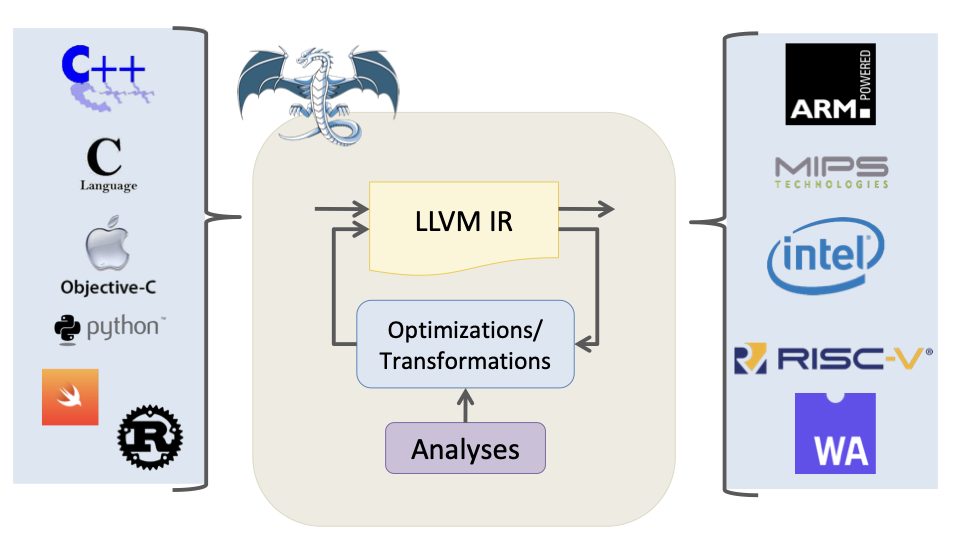
\includegraphics[scale=0.4]{llvm.png}
 
  \caption{The LLVM compiler infrastructure centered around LLVM IR}
  \label{fig:your-label}
\end{figure}

Due to the current complexity and size of LLVM, full verification of the entire compilation toolchain is unlikely. At the same time, developers continuously discover bugs in LLVM. Because of its extensibility, a bug in LLVM can affect any language whose compiler relies on it and thereby compromise the correctness of compiled programs across multiple programming languages.
In particular, LLVM is used in the compilation of Lean, which serves not only as a programming language but  as a theorem prover. In Lean, the compiler is employed in proofs by reflection, where a computation  executed, and the result is reflected back into a formal proof. The correctness of both the computation and the resulting proof thus hinge on the trustworthiness of the compiler. A bug in LLVM could therefore undermine the trustworthiness of the guarantees provided by these proofs. Similarly, the Rust compiler uses LLVM in its standard compilation pipeline.[quote andy talk] While verification efforts focus on ensuring safety and correctness at the Rust language level, once a program is lowered to LLVM IR, the correctness of the final machine code relies entirely on the reliability of the LLVM toolchain. This makes the LLVM ecosystem an interesting and important target for the application of formal methods and verification.

\begin{figure}[htbp]
  \centering
  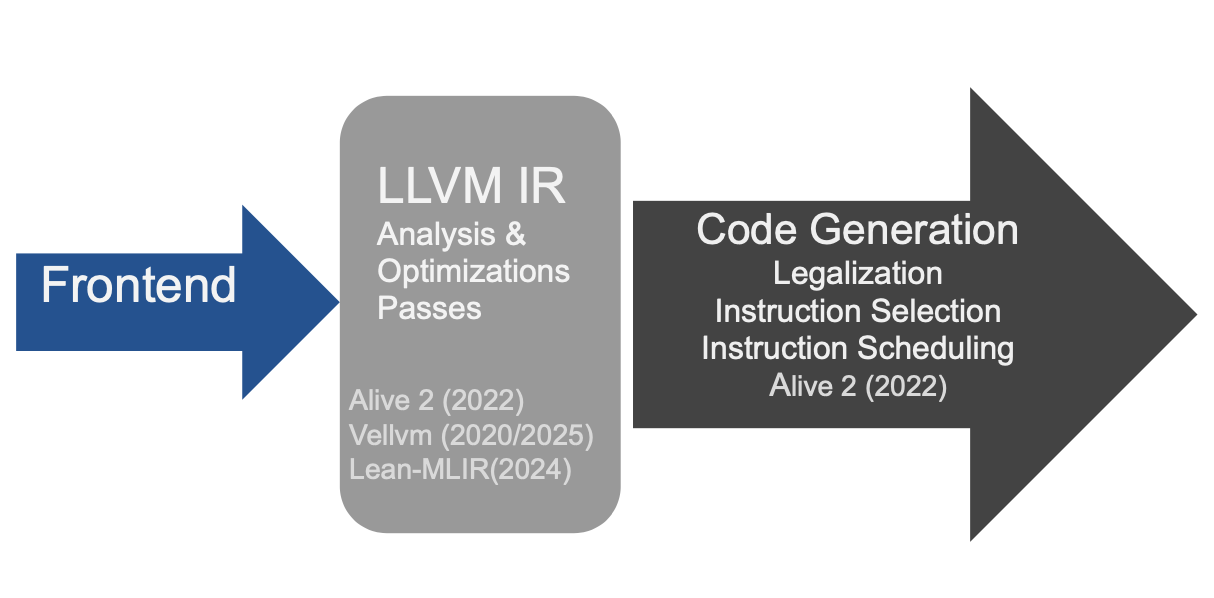
\includegraphics[scale=0.35]{verification_efforts_intro.png}
  \caption{Verification efforts within the LLVM ecosystem}
  \label{fig:your-label}
\end{figure}

At the time of this thesis there exist verification efforts that target the LLVM ecosystem around LLVM IR e.g. the Alive2 project, which verifies optimizations employed in the LLVM InstCombine pass, an IR-to-IR optimizations pass. [Quote]
Existing projects focus primarily on properties of the higher-level LLVM stack and rewrites within LLVM IR itself and do not focus on the lower ends. Meanwhile, backends and low-level assembly code transformation are known to be the most bug-dense compiler components. (quote peek paper). 

Therefore, to counteract this gap and with an eye towards integrating modular and extensible formal verification into the LLVM ecosystem, this thesis implements a pass from LLVM IR to RISC-V that applies verified instruction selection. Additionally, we implement a RISC-V peephole optimization pass as well as formally proven LLVM-IR optimizations. The experience and tooling gained during this implementation can be ported to other compiler components and passes.

Our instruction selection pipeline lowers LLVM IR, under certain constraints on the input program, and translates it into RISC-V assembly targeting a 64-bit architecture. The scope of this thesis focuses on the pure arithmetic subset of LLVM IR instructions, including bitwise operations and integer arithmetic. We operate on legalized LLVM IR, and therefore restrict our attention to 64-bit instructions compatible with the RISC-V 64-bit target.
[Note to self: it might be interesting to implement the legalization myself because atm this really restrict the programs I can modell, actually really want to change this]
The design of our instruction selection pipeline as individual rewriting patterns emphasizes extensibility as it enables the addition of new instruction lowering patterns and optimizations without requiring users to engage or modify complex verified algorithms typical of other formal verification projects e.g CompCert. 
Our proofs in Lean ensure that the generated machine code faithfully preserves the semantics of the original LLVM IR, including the handling of LLVM’s poison values [see Chapter: to do refer to the chaptre where I talk about poison values].

By additionally proposing a verified peephole optimization pass for the generated RISC-V machine code,  we introduce verified assembly-level optimizations in our work and eliminate potential inefficiencies introduced during instruction selection. Similarly, we implement a fully verified peephole rewriting pass for LLVM-IR, which has not been implemented yet. Peephole optimizations are small, local transformations that replace short sequences of assembly instructions with semantically equivalent but more efficient ones [quote Peephole paper]. The code size of the Peephole Rewritter in LLVM (10\% of the IR transforming code base) suggests their relevance within the LLVM toolchain. [quote SSA paper].

\textbf{Methodology}
Motivated by the goal of implementing a formally verified instruction selection pass and peephole optimizations pass for LLVM IR and RISC-V in a flexible and modular manner, we use Lean-MLIR as the foundation for our work.

Lean-MLIR is a project that provides the  \textit{Lean-MLIR(X)}  framework for modeling SSA-based compiler intermediate representations (IRs) within the Lean theorem prover. In Static Single Assignment (SSA) form, each variable is assigned exactly once, simplifying program analysis and transformation. Lean-MLIR enables rigorous formal reasoning about these IR's using Lean.

MLIR, part of the LLVM ecosystem, is a compiler infrastructure that supports multiple domain-specific, SSA-based IR's (dialects) within a unified framework. This hybrid IR model allows different parts of a program to be represented at varying levels of abstraction, enabling optimizations to be applied where the most relevant semantic information is available. MLIR showcases the power of a modular IR design.

\begin{figure}[ht]
\centering
\begin{lstlisting}[language=mlir, basicstyle=\ttfamily\small]
module {
  func.func @simple_add(%arg0: i32, %arg1: i32) -> i32 {
    %sum = arith.addi %arg0, %arg1 : i32
    return %sum : i32
  }
}

\end{lstlisting}
\caption{ MLIR code using the \texttt{arith}, \texttt{func},  and \texttt{built.in} dialects to perform integer addition. The \texttt{arith} dialect holds integer mathematical operations, the \texttt{func} dialect contains function abstractions. The \texttt{built.in} dialect contains standart operations used across many domains.}
\label{fig:mlir-addition}
\end{figure}

We build on the existing LLVM IR dialect in Lean-MLIR and implement a custom RISC-V dialect, expressing the core of our instruction selection as a lowering transformation between these two dialects. To reason about the correctness of our instruction selection, we rely on precise formal semantics for both the source and target languages. Formal semantics assigns rigorous, mathematically defined meaning to each instruction, enabling us to reason about transformations in a mathematically rigorous manner using Lean. For LLVM IR, we leverage the existing semantic model provided by Lean-MLIR. For RISC-V, we rely on the formal specification developed in the Sail project, which mechanizes instruction set architectures in Sail, a domain-specific language. 

To implement our verified peephole optimization passes, we analyze and adapt patterns used in LLVM passes such as Inst Combine and DagCombine.

For verification, we leverage and extend Lean’s native support for bit vector reasoning and its integration of bv\_decide, the first fully verified SMT solver embedded in a theorem prover. Compared to projects like CompCert, we aim for significantly more automation when reasoning about bit-level computations. 

\textbf{Contributions }

By providing a verified instruction selection pass from a subset of LLVM IR to RISC-V 64-bit architecture, along with a subsequent peephole optimization pass, we propose a method for enabling trustworthy code generation from LLVM IR in its dialect form to Risc-V. By mechanizing our implementation in the Lean theorem prover, we achieve formal correctness guarantees and provide an example that can be adapted to other machine targets. For developers who prefer not to rely on the complex and opaque LLVM backend, our pass offers a formally verified alternative for lowering to machine code, while remaining seamlessly integrable into the LLVM ecosystem by modeling it as an applicable pass over the LLVM IR dialect. Our pipeline concretizes the rewrites typically hidden within multiple stages of the complex LLVM backends. Moreover, our design of modeling instruction selection as simple rewrites across two languages can be easily extended with new rewrites.
Our peephole optimization pass for LLVM IR and RISC-V additionally implement new verified optimization passes.

In addition, we provide a command-line interface for our instruction selection pass, inspired by the LLVM optimizer. This interface allows developers to visualize the output of our pipeline and display the applied transformation.
[NOTE: not yet working, unhappy with the printing, I am not yet sure if we can print Risc-V SSA properly.]

Explicitly, we contribute the following:

- Implement a RISCV-V dialect in Lean-MLIR which modells RISC-V assembly operations in Lean. The RISC-V dialect in Lean is given with proofs that the dialect exactly implement the semantics as specified by the Sail RISCV modell for 64-bit address space processors.

- Implement a LLVM and Risc-V hybrid dialect in Lean-MLIR, which allows to implement instruction lowerings as rewrites within the dialect including conversion cast analog to MLIR.

- Implement a legalization pass that converts LLVM IR with width ranging from 8 to 64-bits into legalized LLVM IR programs only operating on 64-bit values. 
[Note: Lie, haven't implemented this but is part of the visiosn but I am not sure that this is even possible in Lean-MLIR atm. I want this because it allows me to lower all the alive test case]

-Design and implement a verified instruction selection pass from the LLVM IR dialect (pure arithmetic fragment) to the RISC-V SSA-assembly-style dialect with instruction selection patterns extracted from LLVM.

- Implement a RISC-V peephole optimization passes that includes XY\% of the optimizations performed by the LLVM backends.
[Note: Lie at the moment because not implemented yet and I therefore cannot state how much we cover, I also am not sure how to extract all of that data yet since my instruction collection is limited]

- Optimizer command line tool \textit{"opt"} for Lean, that processes LLVM IR files and allows to apply the instruction lowering pass and optimization passes by providing the corresponding flag.
[Note: Also, it doesnt work yet because the input is not LLVM IR files but only regions in LLVM IR dialect style and not even all of the syntax is supported yet. I claim the previous opt tool used wrong MLIR syntax].

- Implement register allocation for the RISC-V SSA-style IR to obtain RISCV-V machine code.
[Note: Lie, not done yet but is part of the vision]

- Assembly Printer that outputs resulting RISC-V machine code.
[note: Lie]
